\begin{frame}{$K^- d \rightarrow n \pi^+ \pi^- "n"$ IM fit for $K^0$ and $\Sigma_{forwrad}$ prod.}
  \label{page:Fit_IM}
  
  \scriptsize
  \begin{itemize}
  \item $K^- d \rightarrow K^0 "n" n_{detected}$ 
  \item $K^- d \rightarrow "n" \pi^{\mp} \Sigma^{\pm}_{forward}$  $\Sigma^{\pm}_{forward} \rightarrow \pi^{\pm} n_{detected}$
  \item $K^- d \rightarrow \pi^{\mp} "\Sigma^{\pm}" n_{detected}$
  \end{itemize}
  
  \tminipageThree{
    \begin{figure}
      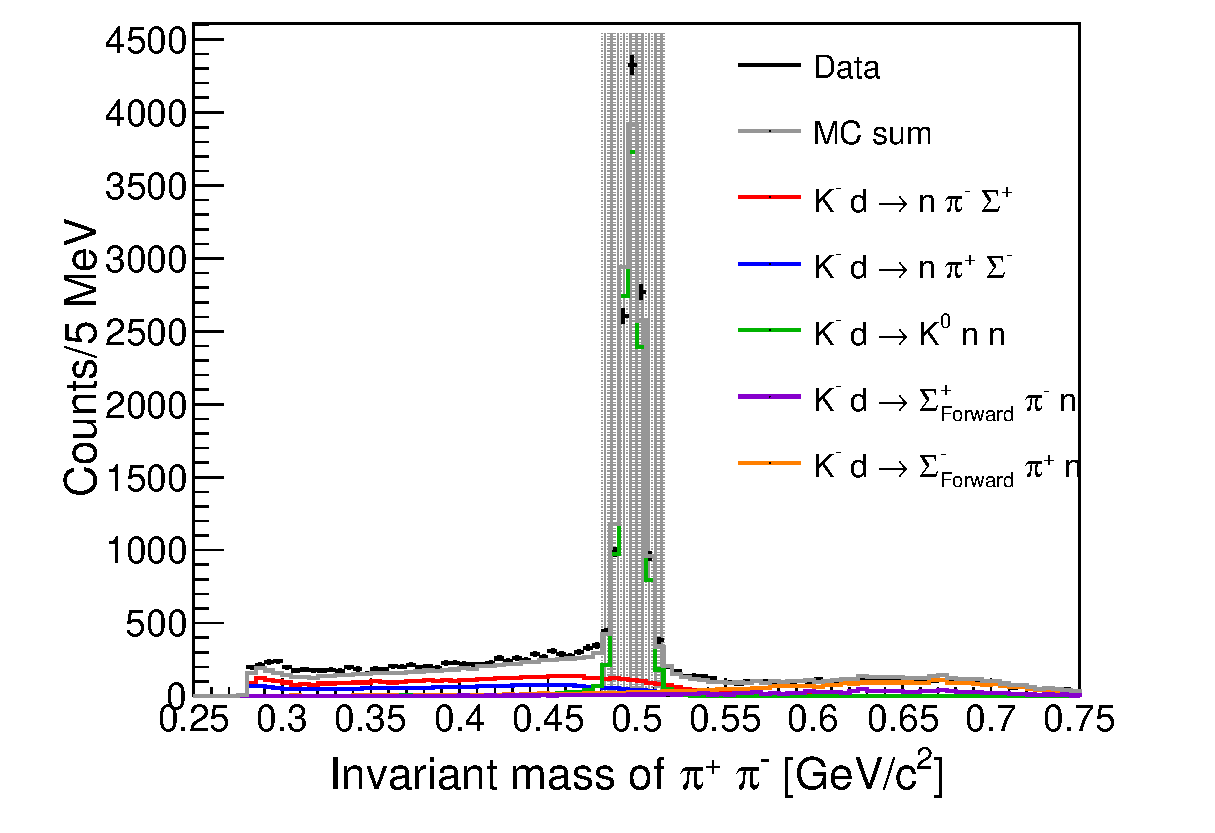
\includegraphics[width=3cm]{../pic/Run78/KN_ana/IM_pipi.eps}
    \end{figure}
  }{
    \begin{figure}
      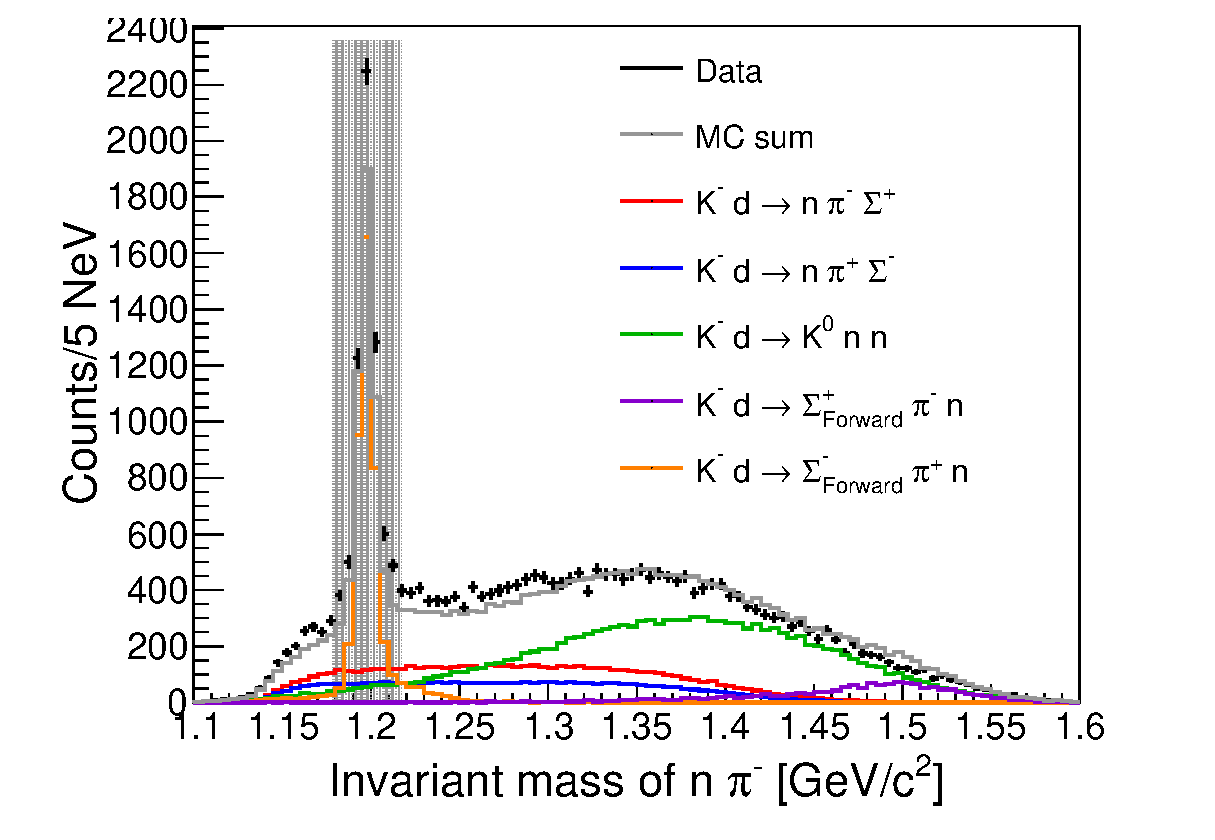
\includegraphics[width=3cm]{../pic/Run78/KN_ana/IM_npim.eps}
    \end{figure}
  }{
    \begin{figure}
      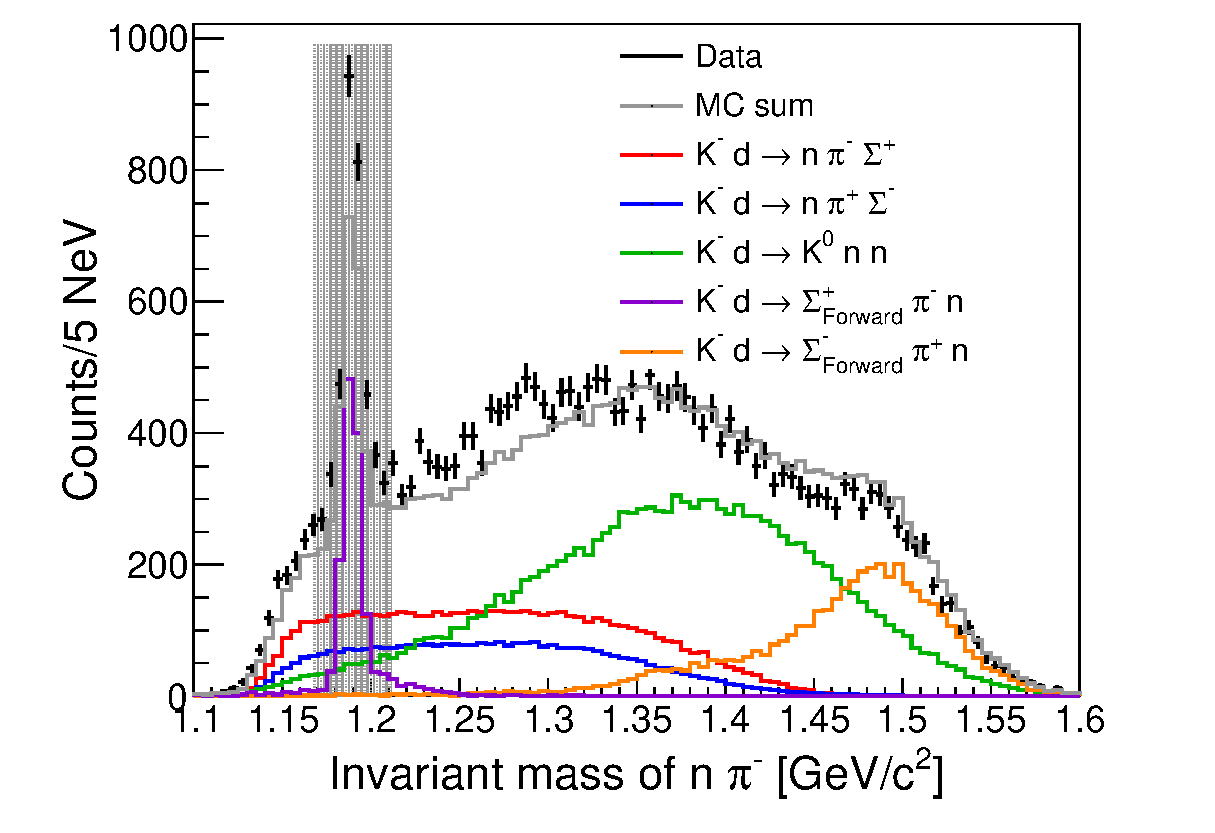
\includegraphics[width=3cm]{../pic/Run78/KN_ana/IM_npip.eps}
    \end{figure}
  }

  \begin{tabular}{cc}
    \begin{minipage}{0.4\hsize}
      \begin{figure}
        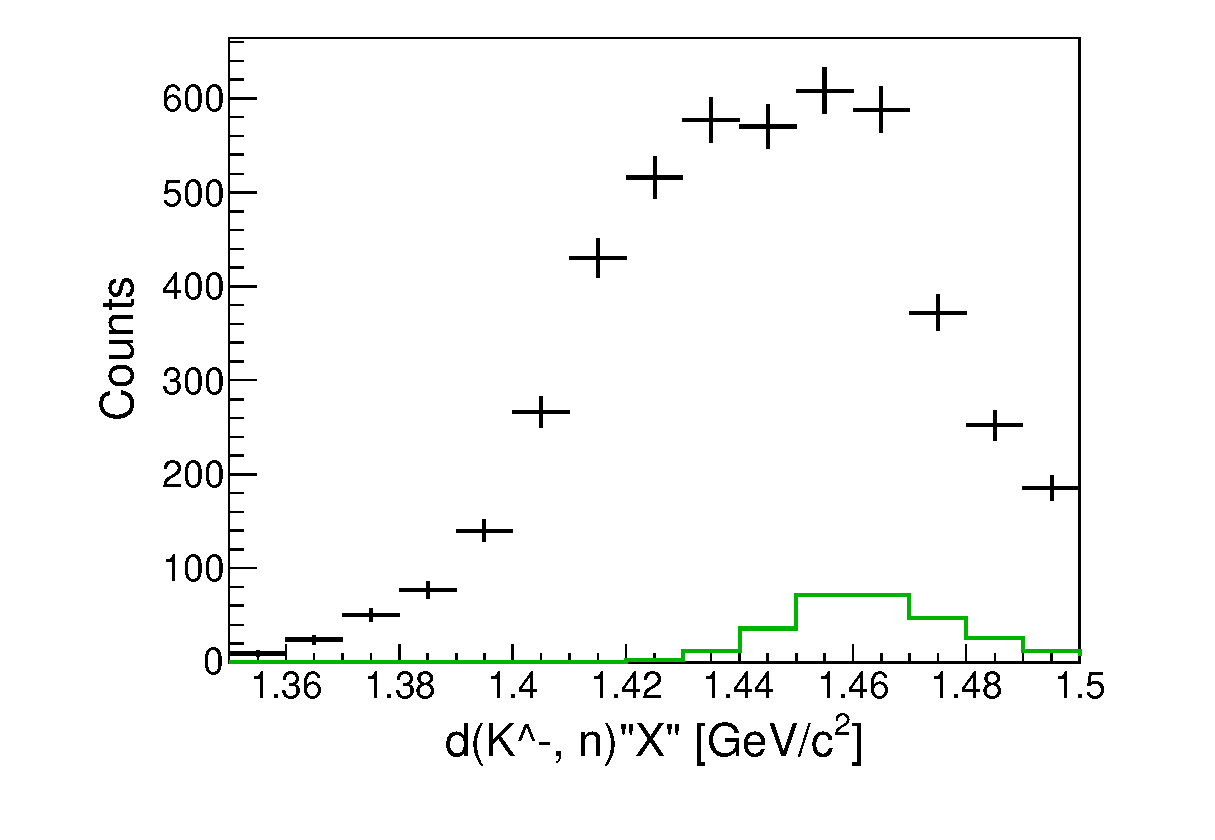
\includegraphics[width=5cm]{../pic/Run78//KN_ana_NC170_2sigma//KN_MM_woAll.eps}
        %% \captionsetup{font=scriptsize}
        %% \caption{
        %%   $K^0$、$\Sigma^{\pm}_{forward}$生成を除いたイベント
        %% }
      \end{figure}
    \end{minipage}
    \begin{minipage}{0.6\hsize}
      \centering
      \scriptsize
      Left figure shows events rejecting $K^0$ and $\Sigma_{forwrad}$ prod. \\
      Gray hatched region indicates rejection region. \\
      Each contamination was estimated by MC sim represented at up figures.\\
      In this spectrum, each $\pi^{\mp}\Sigma^{\pm}$ mode are included,\\
      which are separated by $d(K^-, n \pi^{\mp})"\Sigma^{\pm}"$ fitting.
%%      左図は$K^0$、$\Sigma_{forward}$生成を除いたイベント。\\
%%      上図の灰色の部分($3\sigma$)で排除している。\\
%%      各反応の混入は上のMCによって見積もられている。\\
%%      これらは$K^-d\rightarrow \pi^{\mp} \Sigma^{\pm} n_{detected}$両方の \\ 荷電モードが含まれる。\\
%%      それらは$d(K^-, n \pi^{\mp})"\Sigma^{\pm}"$の\\フィッティングによって分離される。
    \end{minipage}
  \end{tabular}
  
\end{frame}
